\documentclass[12pt]{article}

\usepackage[a4paper, margin=0.5in]{geometry}
\usepackage{anyfontsize}
\usepackage{xcolor}
\usepackage{graphicx}
\usepackage{setspace}
\usepackage{hyperref}
\usepackage[backend=biber]{biblatex}
\usepackage{float}
\usepackage{svg}
\usepackage{xepersian}
\usepackage{amssymb}
\usepackage{amsmath}
\usepackage{enumitem}
\usepackage{caption}
\usepackage{bigints}
\hypersetup{colorlinks,urlcolor=blue}
%\settextfont[Scale=1.1]{Far.Mitra}

\settextfont[Scale=1.0, Size=14pt]{B Nazanin}
\defpersianfont\persiantitlefont[Scale=1.0, Size=18pt]{B Titr}
\setlatintextfont[Scale=1.0, Size=12pt]{Times New Roman}
\deflatinfont\englishtitlefont[Scale=1.0, Size=16pt]{Times New Roman Bold}
\definecolor{mediumpersianblue}{rgb}{0.0, 0.4, 0.65}
\usepackage[backend=biber]{biblatex}
\addbibresource{references.bib}


\def\labelitemi{$\diamond$}
\def\labelitemii{$\ast$}


\begin{document}
	\linespread{3}
	\setstretch{1.5}
	

	\begin{minipage}[t]{0.7\textwidth}
		
		{\huge\textcolor{mediumpersianblue!70!black}{\title\textbf{{ رباتیک}}}}\\[4pt]
		
	\end{minipage}
	\hfil
	\begin{minipage}[t]{0.15\textwidth}
		\centering
		
\includegraphics[width=0.9\linewidth]{pics/logo.png}\\[6pt]
		{\small پاییز ۱۴۰۴}
	\end{minipage}
	
	
	
	{
		
		\Large{تمرین سوم}
		
		\large مرتضی ملکی‌نژاد شوشتری - ۸۱۰۱۰۴۲۵۶ 
		
		
	}
	
	\vspace{1.2cm}
	
	
	
	\vspace{0.3cm}
	\hrule 
	\vspace{0.6cm}
	
	\section{ژاکوبین ربات چهار درجه آزادی اسکارا}
	باید مقادیر
	 $\vec{e}$
	 و 
	 $\vec{r}$
	 را یافت.
	 \begin{latin}
	 	~\\
	 	$
	 	\vec{e_1} = -\vec{k} , \vec{e_2} = -\vec{k}, \vec{e_3} = -\vec{k}, \vec{e_4} = 0
	 	$
	 	\\
	 	$
	 	\vec{r_3} = -d_4\vec{k} , \vec{r_2} = l_2 \vec{j} + \vec{r_3}, \vec{r_1} = -sin(\theta_2) l_1 \vec{i} + cos(\theta_2 )l_1 \vec{j} + \vec{r_2} 
	 	$
	 	\\\\
	 	$
	 	\Rightarrow
	 	e_1 = e_2 = e_3 \begin{bmatrix}
	 		0 \\
	 		0 \\
	 		-1 \\
	 	\end{bmatrix}
	   e_4 = \begin{bmatrix}
	   	0 \\
	   	0 \\
	   	1
	   \end{bmatrix}	   
	 	r_3 = \begin{bmatrix}
	 		0 \\
	 		0 \\
	 		-d_4
	 	\end{bmatrix}
	 	r_2 = \begin{bmatrix}
	 		0 \\
	 		l_2 \\
	 		-d_4
	 	\end{bmatrix}
	 	r_1 = \begin{bmatrix}
	 		-sin(\theta_2)l_1 \\
	 		cos(\theta_2)l_1 + l_2 \\
	 		-d_4
	 	\end{bmatrix}
	 	$
	 \end{latin}
	 پس برای ژاکوبین داریم: (دو سطر اول صفر هستند و با توجه به فرمول $\phi$ در ربات \lr{SCARA} چون ربات چهار درجه آزادی دارد،‌ژاکوبین چهار در چهار برای آن درست تر است. برای همین و طبق فرمول اثبات شده در جزوه دو سطر اول حذف شدند.)
	 \begin{latin}
	 	$
	 	J = \begin{bmatrix}
	 		1 & 1 & 1 & 0 \\
	 		-l2 -l1 cos \theta_2  & -l_2 & 0 & 0 \\
	 		l1 sin \theta_2 & 0 & 0 & 0 \\
	 		0 & 0 & 0 &  1 \\
	 	\end{bmatrix}
	 	$
	 \end{latin}
	 
	 باتوجه به تنظیمات داده شده،‌مقدار ژاکوبین برابر است با:
	 	 \begin{latin}
	 	$
	 	J = \begin{bmatrix}
	 		1 & 1 & 1 & 0 \\
	 		 -0.5  & -1 & 0 & 0 \\
	 		\cfrac{\sqrt{3}}{2}  & 0 & 0 & 0 \\
	 		0 & 0 & 0 &  1 \\
	 	\end{bmatrix}
	 	$
	 \end{latin}
	 برای محاسبه 
	 سرعت برداری
	 داریم:
	 \begin{latin}
	 	$
	 	\vec{t} = J\dot{\theta} \Rightarrow \dot{\theta} = J^{-1}\vec{t} = 
	 	\begin{bmatrix}
	 		0 & 0 & \tfrac{2\sqrt3}{3} & 0 \\
	 		0 & -1 & -\tfrac{\sqrt3}{3} & 0 \\
	 		1 & 1 & -\tfrac{\sqrt3}{3} & 0 \\
	 		0 & 0 & 0 & 1 \\
	 	\end{bmatrix}
	 	\begin{bmatrix}
	 		1.3 \\
	 		-1.15 \\
	 		\cfrac{\sqrt{3}}{20} \\
	 		0
	 	\end{bmatrix}
	 	\Rightarrow
	 	\dot{\theta}
	 	= 
	 	\begin{bmatrix}
	 		0.1 \\
	 		1.1 \\
	 		0.1 \\
	 		0
	 	\end{bmatrix}
	 		 	$
	 \end{latin}
	 \section{تکینگی \lr{Puma 560}}
 {
 \centering
 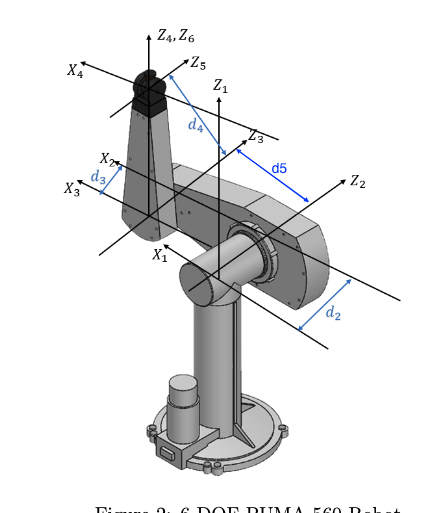
\includegraphics[trim=0 10 0 0, clip, width=0.5\textwidth]{pics/q2_robot.png}
 \captionof{figure}{محورهای ربات. در تصویر سوال مقدار $d_5$ ذکر نشده است.}
 }

        	در شکل مقدار طول بازوها (فاصله محورهای دوران بازو) به ترتیب 
        	$l_1$ 
        	و 
        	$l_2$
        	درنظر گرفته شد. همچنین محورهای 
        	$x_5, x_6, z_7$
        	و 
        	$x_7$
        	رسم نشده‌اند. که
        	$z_7$
        	برابر با راستای موجود $x_4$ درنظر گرفته شد و به این ترتیب 
        	$x_5$
        	برابر با راستای موجود
        	$x_4$
        	و 
        	$x_6$
        	برابر با راستای موجود 
        	$z_5$
        	می‌شود. مقدار $x_7$ نیز برابر با راستای موجود $x_4$ درنظر گرفته شد.
        	        \begin{table}[ht]
        		\centering
	\caption{پارامترهای \lr{DH} ربات \lr{Puma 560}}
	\label{tab:q2-dh}
	\begin{latin}
		\begin{tabular}{c | ccc c}
			number & $a$ & $b$ & $\alpha$ & $\theta$ \\
			\hline
			1 & 0 & $d_2$ & $\cfrac{\pi}{2}$  & $\theta_1$ \\
			2 & $l_1$ &  0 &  0 & $\theta_2$ \\
			3 & 0  & $l_2$ &  $-\cfrac{\pi}{2}$ &  $\theta_3$ \\
			4 & 0 & 0  & $\cfrac{\pi}{2}$ & $\theta_4$ \\
			5 & 0 & 0 & $-\cfrac{\pi}{2}$ & $\cfrac{\pi}{2} + \theta_5$ \\
			6 & 0 & 0 & $-\cfrac{\pi}{2} $ & $\theta_6 - \cfrac{\pi}{2} $ \\
		\end{tabular}
	\end{latin}
\end{table}
برای ژاکوبین داریم:
%\begin{latin}
%	$
%	T_i = \begin{bmatrix}
%		\cos\theta_i & -\sin\theta_i\cos\alpha_{i} & \sin\theta_i\sin\alpha_{i} & a_{i}\cos\theta_i \\
%		\sin\theta_i & \cos\theta_i\cos\alpha_{i} & -\cos\theta_i\sin\alpha_{i} & a_{i}\sin\theta_i \\
%		0 & \sin\alpha_{i} & \cos\alpha_{i} & b_i \\
%		0 & 0 & 0 & 1
%	\end{bmatrix}
%	\Rightarrow
%	T_1 = \begin{bmatrix}
%		cos \theta_1  & 0 & sin \theta_1 & 0\\
%		sin \theta_1 & 0 & -cos \theta_1 & 0 \\
%		0 & 1 & 0 & d_2 \\
%		0 & 0 & 0 & 1\\
%	\end{bmatrix}
%	$
%	\\
%	$
%	T_2 = \begin{bmatrix}
%		cos \theta_2  & -sin \theta_2 & 0 & l_1 cos \theta_2 \\
%sin \theta_2 & cos \theta_2 & 0 & l1 sin \theta_2 \\
%0 & 0 & 1 & 0 \\
%0 & 0 & 0 & 1\\
%	\end{bmatrix}
%	T_3 = \begin{bmatrix}
%		cos \theta_3  & 0 & -sin \theta_3 & 0\\
%		sin \theta_3 & 0 & cos \theta_3  & 0 \\
%		0 & -1 & 0 & 0 \\
%		0 & 0 & 0 & 1\\
%	\end{bmatrix}
%	T_4 = \begin{bmatrix}
%		cos \theta_4  & 0 & -sin \theta_4 & 0\\
%		sin \theta_4 & 0 & -cos \theta_4 & 0 \\
%		0 & 0 & 1 & 0 \\
%		0 & 0 & 0 & 1\\
%	\end{bmatrix}
%	$
%\end{latin}
%کامل حل نشده است.

\begin{latin}
	~\\
	$
	e_1 = \begin{bmatrix}
		0 \\
		0 \\
		1\\
	\end{bmatrix}
	e_2 = \begin{bmatrix}
		0 \\
		-1 \\
		0
	\end{bmatrix}
	e_3 = \begin{bmatrix}
	0 \\
	-1 \\
	0 \\
\end{bmatrix}
	e_4 = \begin{bmatrix}
	0 \\
	0\\
	1
\end{bmatrix}
	e_5 = \begin{bmatrix}
	0 \\
	-1\\
	0
\end{bmatrix}
	e_6 = \begin{bmatrix}
	0 \\
	0\\
	1
\end{bmatrix}
	$
	\\
	$
	r_6 = r_5 = \begin{bmatrix}
		0 \\
		0 \\
		0
	\end{bmatrix}
	r_3 = r_4 = \begin{bmatrix}
		0 \\
		0 \\
		l_2
	\end{bmatrix}
		r_2 = r_3 +  \begin{bmatrix}
		0 \\
		l_1 \\
		0
	\end{bmatrix}
	r_1 = r_2 + \begin{bmatrix}
		d_3 - d_2 \\
		0 \\
		0
	\end{bmatrix}
	$
\end{latin}
پس داریم:
\begin{latin}
	$
	J = \begin{bmatrix}
		0 & 0 & 0 & 0 & 0 & 0 \\
		0 & -1 & 0 & -1 & -1 & 0   \\
		1 & 0 & 1 & 0 & 0 & 1 \\
		0 & 0 & 0 & 0 & -l_2 & -l-1  \\
		0 & 0 & 0 & 0 & 0 &  d_2 - d_3 \\
		0 & 0 & 0 & 0 & 0 & 0 \\
	\end{bmatrix}
	$
\end{latin}
 بخش تکینگی حل نشده است.
\section{حساسیت سینماتیکی}
\begin{itemize}


{
\centering
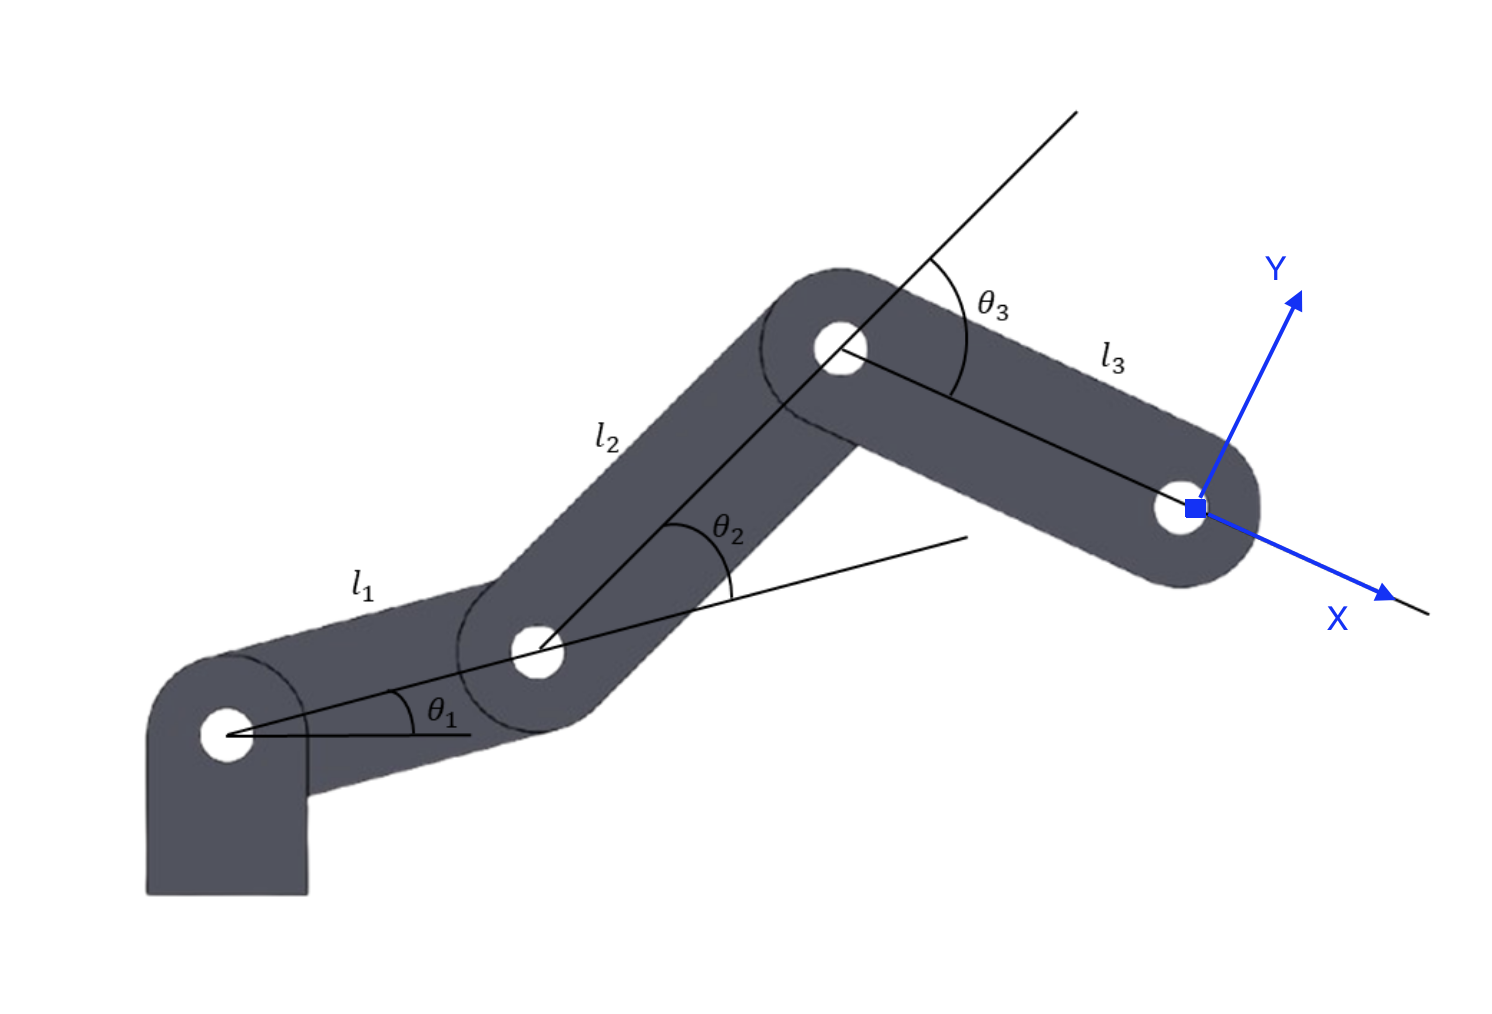
\includegraphics[width=0.8\textwidth]{pics/q3_robot.png}
\captionof{figure}{ربات مورد نظر همراه با محورهای مختصات مجری نهایی}
}
\item 
محورها همه در جهت \lr{Z} هستند.	همچنین برای محاسبه بردار های 
\lr{r}
باید بتوان زاویه را با افق حساب کرد. برای هر محور داریم:

\begin{latin}
	$
	\theta_1' = \theta_1 \qquad \theta_2' = \theta_1 + \theta_2 \qquad \theta_3' = \theta_1 + \theta_2 - \theta_3
	$
\end{latin}
\begin{latin}
	$
	e_1 = e_2 = e_3 = \vec{k}
	$
	\\\\
	$
	r_3 = \begin{bmatrix}
	-l_3cos \theta_3' \\
	-l_3sin \theta_3' \\
	0
	\end{bmatrix}
	r_2 = r_3 + \begin{bmatrix}
		- l_2 cos \theta_2'  \\
		-l_2 sin \theta_2'  \\
		0
	\end{bmatrix}
	r_1 =  r_2 + \begin{bmatrix}
		-l_1 cos \theta_1' \\
		-l_1 sin \theta_1' \\
		0
	\end{bmatrix}
	$
\end{latin}
با جلو رفتن طبق فرمول مرسوم ژاکوبین یک ماتریس شش در شش بدست می‌آید منتها این یک ربات با سه درجه آزادی است و شش درجه نیست. با نگاه به شکل ربات می‌توان دید که متغیرهای آزاد این ربات 
\lr{x, y}
و 
$\phi$
می‌باشد. یعنی در ماتریس ژاکوبین دو سطر اول (زوایای دیگر راستاها) و سطر آخر (برای راستای \lr{z} همواره صفر است و می‌توان آن را ننوشت) 
\begin{latin}
	$
	J = \begin{bmatrix}
		1 & 1 & 1 \\
	 l3 sin \theta_3' +  l2 sin \theta_2 '   +	l1 sin \theta_1'  & l3 sin \theta_3' +  l2 sin \theta_3'   & l3 sin \theta_3' \\
		 l3 cos \theta_3' +  l2 cos \theta_2 '   + l1 cos \theta_1' & l3 cos \theta_3' +  l2 cos \theta_2 '  & l3 cos \theta_3'   \\
	\end{bmatrix}
	$
\end{latin}
\item 
\begin{latin}
	$
	\theta_1' = 75 \quad \theta_2' = 105 \quad \theta_3' = 35 \Rightarrow
	J \approx \begin{bmatrix}
		1  &  1 & 1 \\
		175 &117 & 40 \\
		93 & 78 & 57 \\
	\end{bmatrix} \Rightarrow JJ^T = \begin{bmatrix}
	3 & 332 & 228 \\
	332 & 45914 & 27681 \\
	228 & 27681 & 17982 \\
	\end{bmatrix}
	$
\end{latin}
می‌توان دید که مقادیر ویژه این ماتریس برابر است با:
\begin{latin}
	$
	\lambda = \begin{pmatrix}
		6.29551976e+04 & 6.67987690e-05 & 9.43802339e+02
	\end{pmatrix} 
	$
\end{latin}
پس مقدار 
$\kappa$
برابر است با:
\begin{latin}
	$
	\kappa = \sqrt{\cfrac{6.29551976e+04}{6.67987690e-05 }} \approx 30,700
	$
\end{latin}
	
\end{itemize}
	\section{ربات سه درجه آزادی}
	{
	\centering
	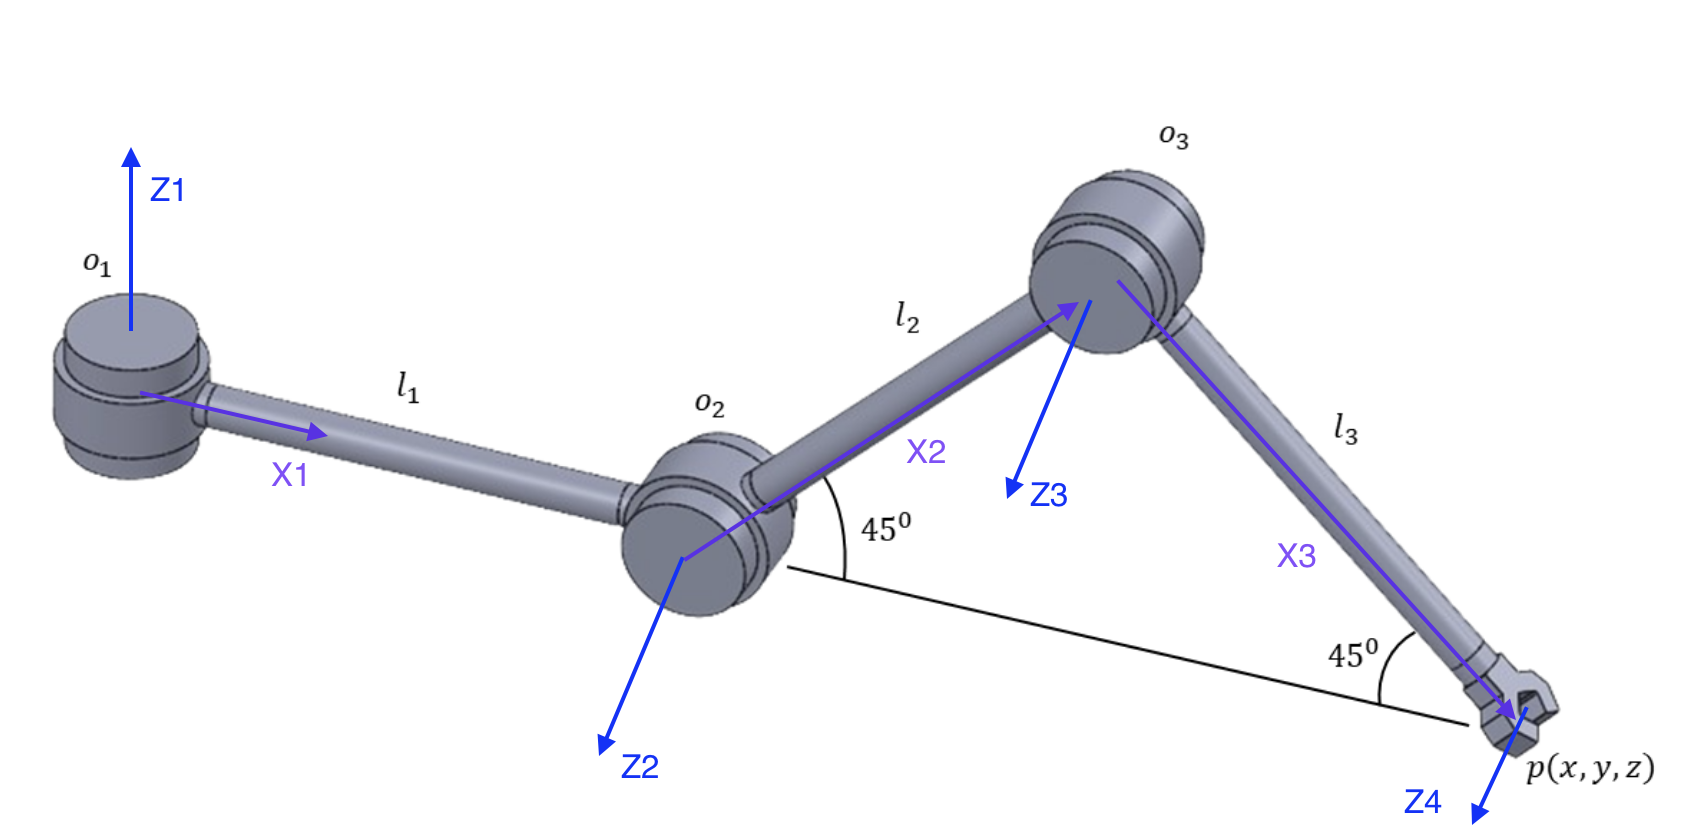
\includegraphics[width=0.7\textwidth]{pics/q4_robot.png}
	\captionof{figure}{محورهای ربات}
	}
\begin{itemize}
\item 

	        	        \begin{table}[ht]
		\centering
		\caption{پارامترهای \lr{DH} ربات سه درجه آزادی سوال چهار}
		\label{tab:q4-dh}
		\begin{latin}
			\begin{tabular}{c | ccc c}
				number & $a$ & $b$ & $\alpha$ & $\theta$ \\
				\hline
				1 &$l_1$ & 0 & $\cfrac{\pi}{2}$ & 0 \\
				2 & $l_2$ & 0 & 0 & $\cfrac{\pi}{4}$ \\
				3 & $l_3$ & 0 & 0 & $-\cfrac{\pi}{2}$ \\
			\end{tabular}
		\end{latin}
	\end{table}
	
	     \begin{table}[ht]
		\centering
		\caption{
			پارامترهای
			 \lr{DH}
			   ربات سه درجه آزادی سوال چهار در حالت کلی}
		\label{tab:q4-dh-gen}
		\begin{latin}
			\begin{tabular}{c | ccc c}
				number & $a$ & $b$ & $\alpha$ & $\theta$ \\
				\hline
				1 &$l_1$ & 0 & $\cfrac{\pi}{2}$ & $\theta_1$ \\
				2 & $l_2$ & 0 & 0 & $\theta_2$ \\
				3 & $l_3$ & 0 & 0 & $\theta_3$ \\
			\end{tabular}
		\end{latin}
	\end{table}
	
	پارامترهای 
	\lr{DH}
	ربات در جدول 
	\ref{tab:q4-dh}
	آمده‌اند.
	\item 
	برای حل 
	\lr{FKP}
	باید ماتریس 
	\lr{transpose}
	هر مفصل را یافت و سپس درهم ضرب کرد.
	\begin{latin}
		$
			T_i = \begin{bmatrix}
	\cos\theta_i & -\sin\theta_i\cos\alpha_{i} & \sin\theta_i\sin\alpha_{i} & a_{i}\cos\theta_i \\
	\sin\theta_i & \cos\theta_i\cos\alpha_{i} & -\cos\theta_i\sin\alpha_{i} & a_{i}\sin\theta_i \\
	0 & \sin\alpha_{i} & \cos\alpha_{i} & b_i \\
	0 & 0 & 0 & 1 \\
\end{bmatrix}
\Rightarrow
T_1 = \begin{bmatrix}
1 & 0 & 0 & l_1 \\
0 & 0 & -1 & 0 \\
0 & 1 & 0 & 0\\
0 & 0 & 0 & 1\\
\end{bmatrix}
,
T_2 = \begin{bmatrix}
\cfrac{\sqrt{2}}{2} & -\cfrac{\sqrt{2}}{2} & 0 & \cfrac{\sqrt{2}}{2} l_2 \\
\cfrac{\sqrt{2}}{2} & \cfrac{\sqrt{2}}{2} & 0 & \cfrac{\sqrt{2}}{2} l_2 \\
	0 & 0 & 1 & 0\\
	0 & 0 & 0 & 1\\
\end{bmatrix}
$
\\
$
T_3 = \begin{bmatrix}
0 &  1 & 0 & 0 \\
-1 & 0 & 0 & -l_3 \\
	0 & 0 & 1 & 0\\
	0 & 0 & 0 & 1\\
\end{bmatrix}
		$
	\end{latin}
	حالا باید این سه ماتریس را درهم ضرب کرد:
	\begin{latin}
		$
		T = T_1 T_2 T_3  = \begin{bmatrix}
			\cfrac{\sqrt{2}}{2} & -\cfrac{\sqrt{2}}{2} & 0 & \cfrac{\sqrt{2}}{2}l_2 + l_1 \\
				0 & 0 & -1 & 0\\
				\cfrac{\sqrt{2}}{2} & \cfrac{\sqrt{2}}{2} & 0 & \cfrac{\sqrt{2}}{2} l_2 \\
					0 & 0 & 0 & 1\\
		\end{bmatrix} 
		*
		T_3
		=
			\begin{bmatrix}
\cfrac{\sqrt{2}}{2} &\cfrac{\sqrt{2}}{2} & 0 & \cfrac{\sqrt{2}}{2} l_3 + \cfrac{\sqrt{2}}{2} l_2 + l_1 \\
	0 & 0 & -1 & 0\\
	-\cfrac{\sqrt{2}}{2} & \cfrac{\sqrt{2}}{2} & 0 & \cfrac{\sqrt{2}}{2} (l_2 - l_3) \\ 
		0 & 0 & 0 & 1\\
		\end{bmatrix} 
		$
	\end{latin}
	می‌دانیم که در این ماتریس، زیر ماتریس سه در سه اول ماتریس دوران است و قسمت سه در یک بعدی مکان مجری نهایی می‌باشد.پس:
	\begin{latin}
		$
		\begin{pmatrix}
			x \\ 
			y \\
			z \\
		\end{pmatrix}
		= 		\begin{pmatrix}
		 \cfrac{\sqrt{2}}{2} l_3 + \cfrac{\sqrt{2}}{2} l_2 + l_1   \\ 
			0 \\
			\cfrac{\sqrt{2}}{2} (l_2 - l_3)  \\
		\end{pmatrix}
		= 	\begin{pmatrix}
			(1 + \sqrt{2})l   \\ 
			0 \\
			0  \\
		\end{pmatrix}
		$
	\end{latin}
	که با شکل ربات منطبق است. (چون ربات سه درجه آزادی دارد، سه متغیر آزاد دارد و سه متغیر دیگر وابسته اند و عملا در معادلات نقشی ندارند برای همین سه متغیر کافی است.)
	
	فرم پارامتری معادلات 
	\lr{FKP}
	برابر است با:
	\begin{latin}
		$
				x = cos \theta_1(l_1  + l_2 cos \theta_2 + l_3 cos (\theta_3 - \theta_2)) \\
		y = l2 sin \theta_2  + l_3 cos (\theta_3 - \theta_2) \\
		z = sin \theta_1 (l_1  + l_2 cos \theta_2 + l_3 cos (\theta_3 - \theta_2)) \\
		$
	\end{latin}
	\item 
	ابتدا معادله مستقیم ربات بصورت پارامتری محاسبه می‌شود.
	\begin{latin}
		$
		x = cos \theta_1(l_1  + l_2 cos \theta_2 + l_3 cos (\theta_3 + \theta_2)) \\
		y = l2 sin \theta_2  + l_3 sin (\theta_2 + \theta_3) = 2l (sin(\theta_2 + \cfrac{\theta_3}{2}) cos ( \cfrac{\theta_3}{2}))\\
		z = sin \theta_1 (l_1  + l_2 cos \theta_2 + l_3 cos (\theta_3 + \theta_2)) 
		= lsin \theta_1 (1 + 2(cos (\theta_2 + \cfrac{\theta_3}{3})) cos ( \cfrac{\theta_3}{2})) \\
				\Rightarrow \theta_1 = arctan(\cfrac{z}{x}) \\
				\Rightarrow
				\theta_2 + \cfrac{\theta_3}{2} = arctan( \cfrac{y}{\cfrac{z}{lsin \theta_1} - 1})
				\\
			\Rightarrow
			y^2 + (\cfrac{z}{l sin \theta_1} - 1)^2 =  4 cos (\cfrac{\theta_3}{2})^2 
			\Rightarrow \theta_3 =2 arccos( \cfrac{\sqrt{y^2 + (\cfrac{z}{l sin \theta_1} - 1)^2 }}{2})
		$
	\end{latin}
	یعنی فرمول‌های نهایی برابرند با:
	\begin{latin}
		$
		\theta_1 = arctan(\cfrac{z}{x}) \\ 
		\theta_3 = 2 arccos( \cfrac{\sqrt{y^2 + (\cfrac{z}{l sin \theta_1} - 1)^2 }}{2}) \\
		 \theta_2 = arctan( \cfrac{y}{\cfrac{z}{lsin \theta_1} - 1}) - \cfrac{\theta_3}{2}\\
		$
	\end{latin}
	\item 
	چون در اینجا معادله 
	\lr{FKP}
	بدست آمده است، می‌توان مستقیم از آن مشتق جزئی گرفت و ماتریس ژاکوبین را پر کرد.
	\begin{latin}
		$
		J = \begin{bmatrix}
		  -sin \theta_1	(l_1  + l_2 cos \theta_2 + l_3 cos (\theta_3 + \theta_2))   &  cos \theta_1( - l_2 sin \theta_2 + l_3 sin (\theta_3 - \theta_2))  &  cos \theta_1(- l_3 sin (\theta_3 + \theta_2)) \\
		  0 & l2cos \theta_2  + l_3 cos (\theta_3 + \theta_2)& l_3 cos (\theta_3 + \theta_2) \\ 
		  cos \theta_1	(l_1  + l_2 cos \theta_2 + l_3 cos (\theta_3 + \theta_2))   &  sin \theta_1( - l_2 sin \theta_2 + l_3 sin (\theta_3 + \theta_2))  &  sin \theta_1(- l_3 sin (\theta_3 + \theta_2)) \\
		\end{bmatrix}
		$
	\end{latin}
	\item 
	باتوجه به متغیرهای داده‌شده داریم:
	\begin{latin}
		$
		\theta_1 = 0 \quad \theta_2 = \cfrac{\pi}{4} \quad \theta_3 = -\cfrac{\pi}{2}
		\Rightarrow
		J = \begin{bmatrix}
			0 & -\sqrt{2}l & \cfrac{\sqrt{2}}{2} l\\
			0 & 0  & -\cfrac{\sqrt{2}}{2} l \\
			l  & 0 & 0 \\
		\end{bmatrix}
		$
	\end{latin}
	\item 
	در نوتبوک 
	\lr{q\_4.ipynb}
	رسم نمودار امده است (برای استفاده از توابع خاص \lr{matplotlib} از هوش مصنوعی کمک گرفته شده است.). نقاطی که دترمینان  کمتر از 
	$0.1$ 
	می‌باشد به عنوان نقاط تکین درنظر گرفته شده‌اند.
	{
	\centering
	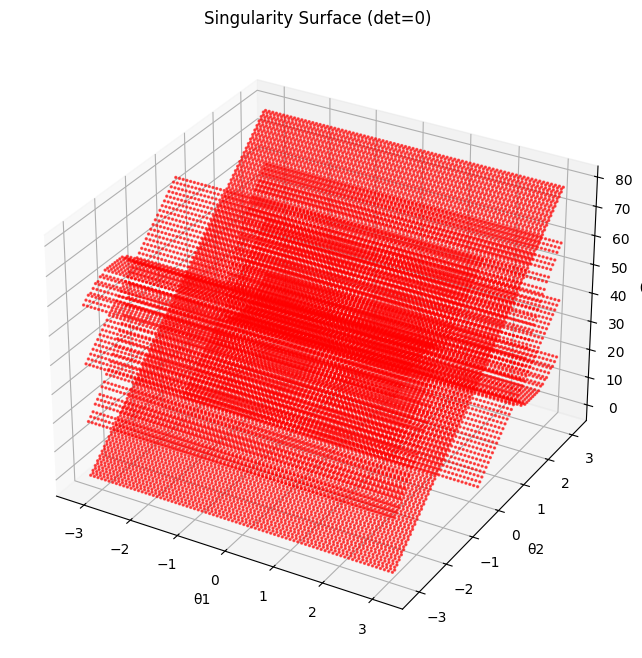
\includegraphics[width=0.7\textwidth]{pics/q4_singular.png}
	\captionof{figure}{نقاط تکین ربات سوال ۴}
	}
	\item 
	برای فضای کاری، می‌توان بصورت هندسی مسئله را حل کرد. اگر مفصل اول در نظر گرفته نشود، دو مفصل باقی مانده شبیه ربات انگشت است که در کلاس حل شد و فضای کاری آن بصورت یک دایره با شعاع 
	\lr{3l}
	است که وسط آن یک دایره به شعاع \lr{l} خالی می‌باشد. حال با درنظر گرفتن مفصل اول، این دایره حول محور \lr{z} دوران پیدا میکند. یعنی شکل نهایی فضای کار یک شکل دونات طور با شعاع بیرونی \lr{3r} و شعاع داخلی \lr{r} است که بیش‌ترین طول این دونات در \lr{2.5r} اتفاق می‌افتد.
	
\end{itemize}

\section{استاتیک ربات \lr{RRPRRR}}
این سوال حل نشده است.
\end{document}